\documentclass[crop=false]{standalone}
\usepackage{standard}
\begin{document}
  \section{Fazit und Aussicht} % (fold)
  \label{sec:conclusion}

    \begin{figure}[b]
      \center
      \begin{subfigure}[b]{0.24\textwidth}
        \center
        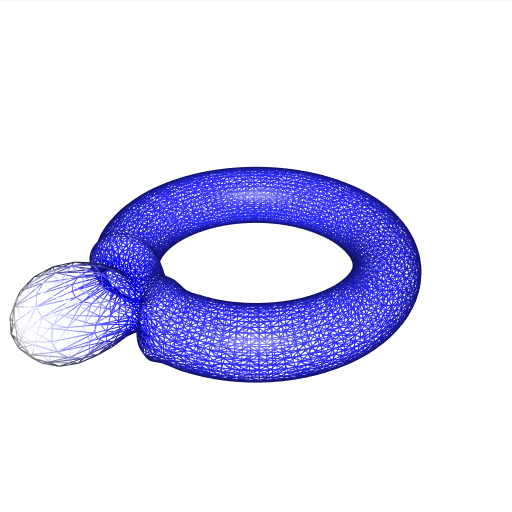
\includegraphics[trim={0.2cm 3.9cm 3.15cm 5.8cm},clip,width=0.95\textwidth]{images/torus_wave_0.png}
        \caption{}
      \end{subfigure}
      \begin{subfigure}[b]{0.24\textwidth}
        \center
        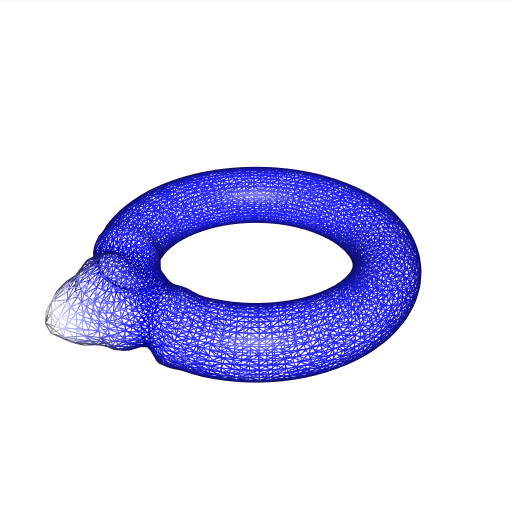
\includegraphics[trim={0.2cm 3.9cm 3.15cm 5.8cm},clip,width=0.95\textwidth]{images/torus_wave_1.png}
        \caption{}
      \end{subfigure}
      \begin{subfigure}[b]{0.24\textwidth}
        \center
        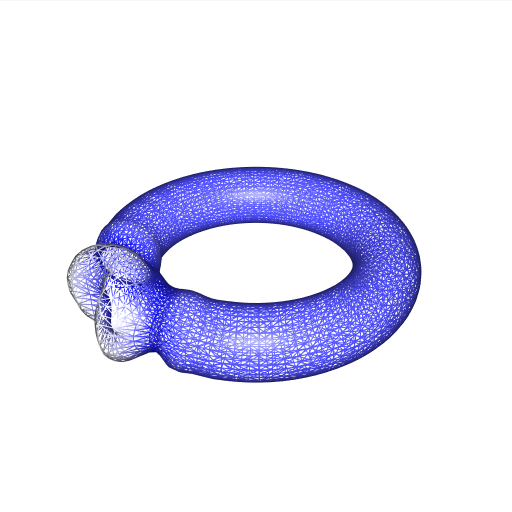
\includegraphics[trim={0.2cm 3.9cm 3.15cm 5.8cm},clip,width=0.95\textwidth]{images/torus_wave_2.png}
        \caption{}
      \end{subfigure}
      \begin{subfigure}[b]{0.24\textwidth}
        \center
        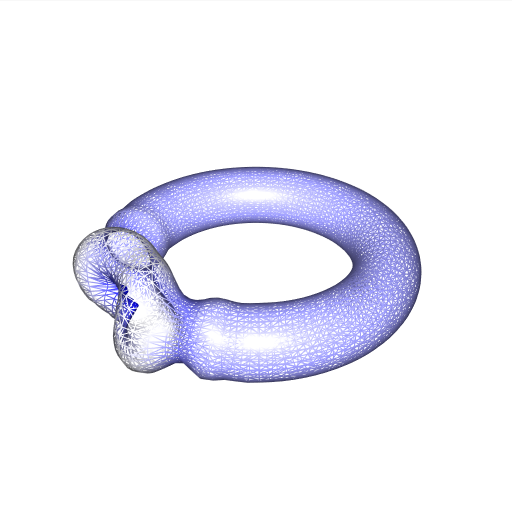
\includegraphics[trim={0.2cm 3.9cm 3.15cm 5.8cm},clip,width=0.95\textwidth]{images/torus_wave_3.png}
        \caption{}
      \end{subfigure}

      \begin{subfigure}[b]{0.24\textwidth}
        \center
        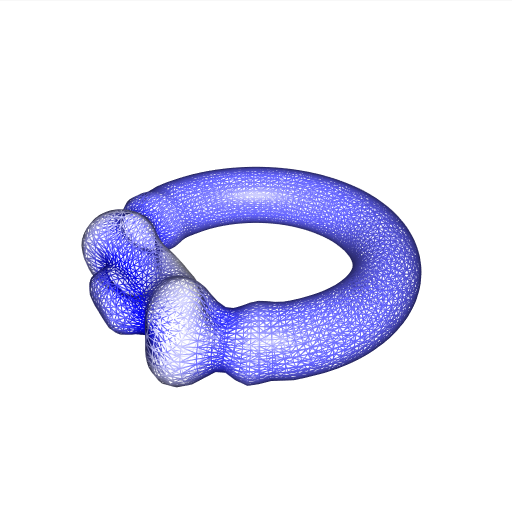
\includegraphics[trim={0.2cm 3.9cm 3.15cm 5.8cm},clip,width=0.95\textwidth]{images/torus_wave_4.png}
        \caption{}
      \end{subfigure}
      \begin{subfigure}[b]{0.24\textwidth}
        \center
        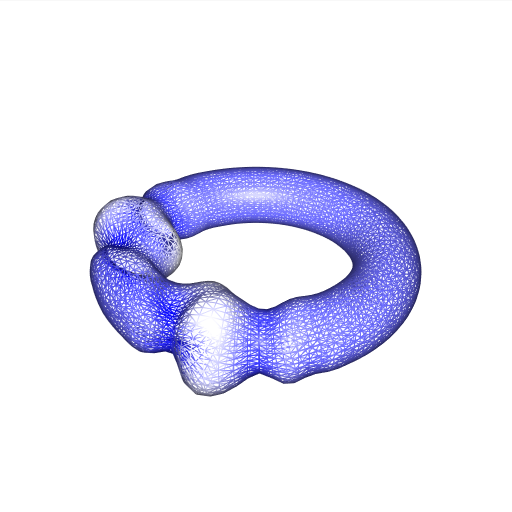
\includegraphics[trim={0.2cm 3.9cm 3.15cm 5.8cm},clip,width=0.95\textwidth]{images/torus_wave_5.png}
        \caption{}
      \end{subfigure}
      \begin{subfigure}[b]{0.24\textwidth}
        \center
        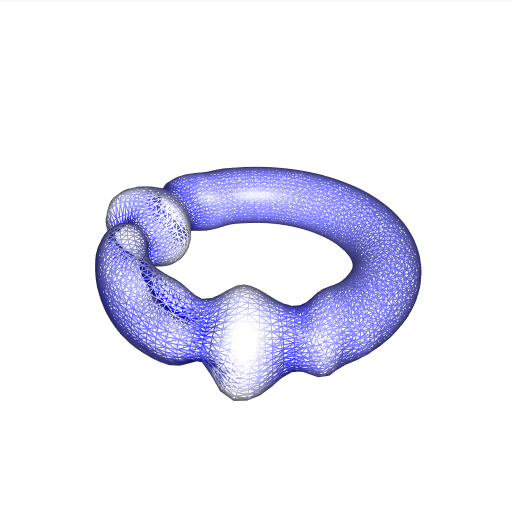
\includegraphics[trim={0.2cm 3.9cm 3.15cm 5.8cm},clip,width=0.95\textwidth]{images/torus_wave_6.png}
        \caption{}
      \end{subfigure}
      \begin{subfigure}[b]{0.24\textwidth}
        \center
        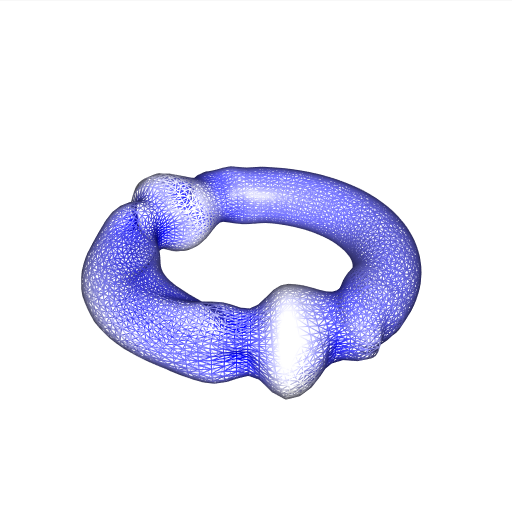
\includegraphics[trim={0.2cm 3.9cm 3.15cm 5.8cm},clip,width=0.95\textwidth]{images/torus_wave_7.png}
        \caption{}
      \end{subfigure}
      \caption[Wellensimulation auf einem Torus]{%
        Die Abbildungen zeigen die Zeitevolution einer Simulation der Wellengleichung auf der gekrümmten Fläche eines Torus.
        Der Torus kann hier als eine Verallgemeinerung von periodischen Randbedingungen auf einem Quadrat angesehen werden.
      }
      \label{fig:torus-wave}
    \end{figure}

    Aus den aufgeführten Ergebnissen können folgende Schlussfolgerungen gezogen werden.
    Die Implementierung der Finite-Elemente-Methode auf der GPU durch die Sprache CUDA brachte einen enormen Performanceanstieg bereits bei kleinen Modellen mit sich.
    Die Grafikkarte eines Computers ist demnach bei der Berechnung eines Zeitschrittes für die Finite-Elemente-Methode der CPU überlegen.
    Die Konstruktion der Systemmatrizen dauert im Vergleich zur Zeitschrittberechnung zu lange.
    Daher ist es empfehlenswert diesen Programmanteil ebenfalls zu parallelisieren.
    Es ist jedoch zu prüfen, ob dieser Schritt auf der GPU oder auf der CPU vorgenommen werden sollte.
    Bei der Konstruktion der Systemmatrizen handelt es sich um ein Reduktionsproblem, welches eine Reduzierung der Datenparallelität zur Folge hat.
    Demzufolge besteht die Möglichkeit, dass eine parallelisierte Implementierung auf der CPU dieses Problem durch eine gesteigerte Taktfrequenz und einen größeren Cache besser lösen könnte.

    Für die Wahl der numerischen Methoden ist eine genaue Analyse der Problemstellung von Nutzen.
    Es gibt kein universelles Verfahren, welches alle Probleme gleichermaßen gut löst.
    Je nach Struktur der dünnbesetzten Systemmatrizen oder der partiellen Differentialgleichungen kann die Wahl einer Methode unterschiedlich geeignet sein.
    Auch hier stellt die Messung der Performance ein adäquates Mittel für die Auswahl der Verfahren dar.
    Für eine detailliertere Behandlung weiterer Verfahren zur Darstellung komplexerer Probleme sei hier auf \cite{Bell2008,Bell2009,Nocedal2006,Logan2007} verwiesen.

    Um die Effizienz des gesamten Verfahrens in der Praxis zu bewerten, sollte dieses anhand realistischer physikalischer Problemstellungen, wie zum Beispiel der Strömungssimulation, gemessen und analysiert werden.
    Die Genauigkeit einer Voraussage hängt von der Diskretisierung des Berechnungsgebietes ab.
    Daher ist es ratsam, einen Algorithmus zur automatischen und adaptiven Gittergenerierung zu verwenden.

    Eine Erweiterung des hier implementierten Verfahrens ist die Berechnung der Wellengleichung auf zweidimensionalen gekrümmten Oberflächen.
    In den Abbildungen \ref{fig:torus-wave} und \ref{fig:sphere-wave} ist dies für einen Torus und eine Kugel veranschaulicht.
    Dies demonstriert, dass die Finite-Elemente-Methode auch auf mathematisch motivierte Probleme anwendbar ist.

    \begin{figure}
      \center
      \begin{subfigure}[b]{0.24\textwidth}
        \center
        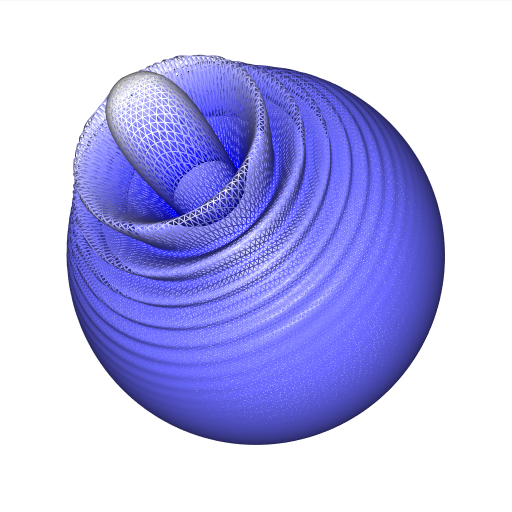
\includegraphics[trim={2.12cm 2.33cm 2.2cm 0cm},clip,width=0.95\textwidth]{images/sphere_wave_0.png}
        \caption{}
      \end{subfigure}
      \begin{subfigure}[b]{0.24\textwidth}
        \center
        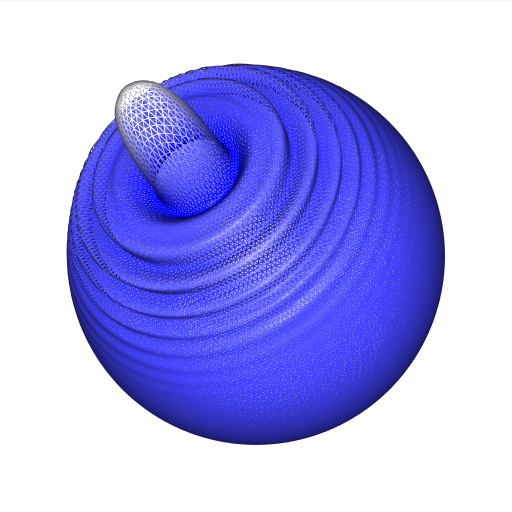
\includegraphics[trim={2.12cm 2.33cm 2.2cm 0cm},clip,width=0.95\textwidth]{images/sphere_wave_1.png}
        \caption{}
      \end{subfigure}
      \begin{subfigure}[b]{0.24\textwidth}
        \center
        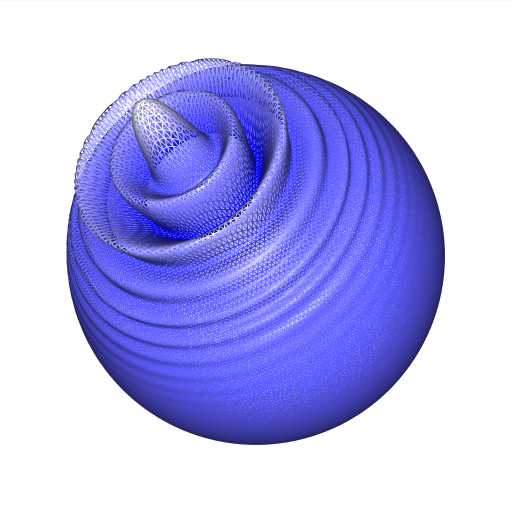
\includegraphics[trim={2.12cm 2.33cm 2.2cm 0cm},clip,width=0.95\textwidth]{images/sphere_wave_2.png}
        \caption{}
      \end{subfigure}
      \begin{subfigure}[b]{0.24\textwidth}
        \center
        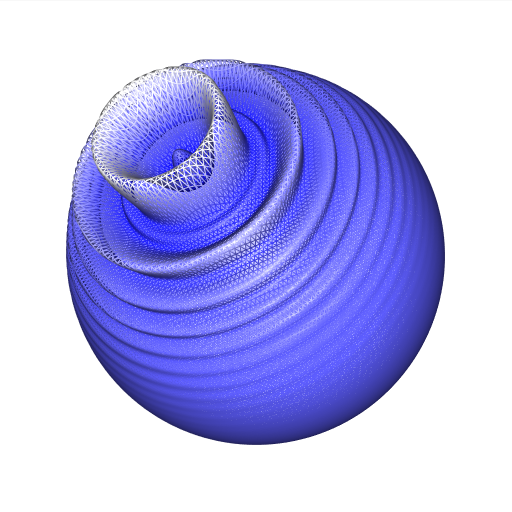
\includegraphics[trim={2.12cm 2.33cm 2.2cm 0cm},clip,width=0.95\textwidth]{images/sphere_wave_3.png}
        \caption{}
      \end{subfigure}

      \begin{subfigure}[b]{0.24\textwidth}
        \center
        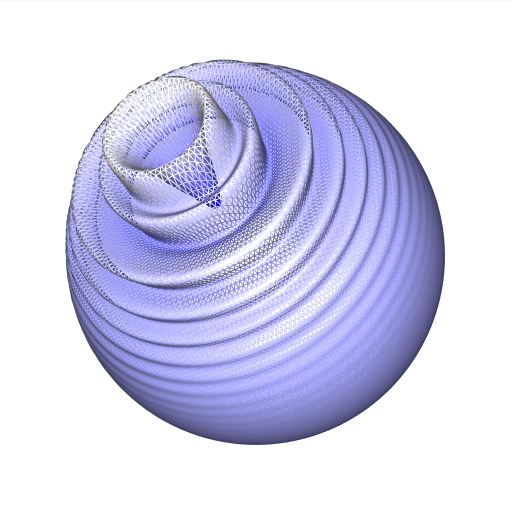
\includegraphics[trim={2.12cm 2.33cm 2.2cm 0cm},clip,width=0.95\textwidth]{images/sphere_wave_4.png}
        \caption{}
      \end{subfigure}
      \begin{subfigure}[b]{0.24\textwidth}
        \center
        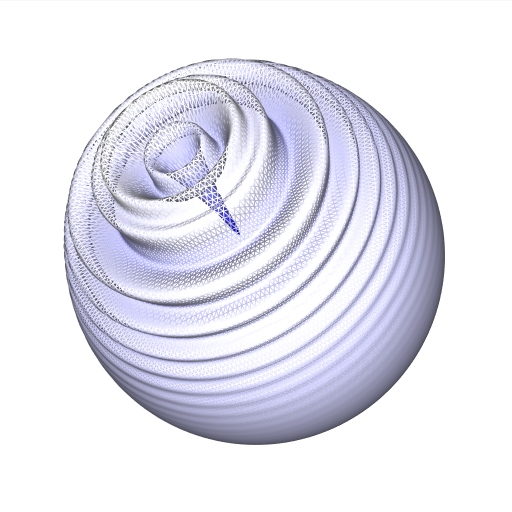
\includegraphics[trim={2.12cm 2.33cm 2.2cm 0cm},clip,width=0.95\textwidth]{images/sphere_wave_5.png}
        \caption{}
      \end{subfigure}
      \begin{subfigure}[b]{0.24\textwidth}
        \center
        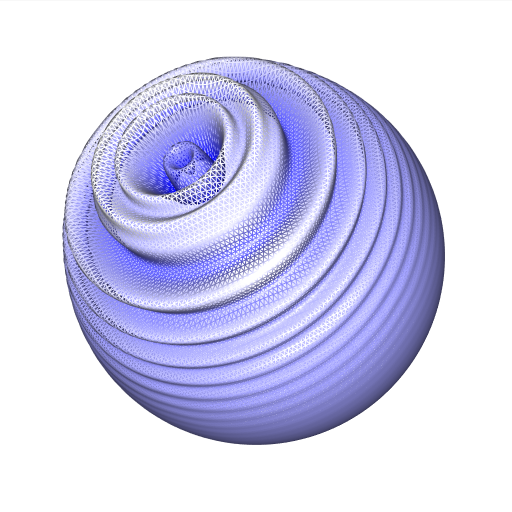
\includegraphics[trim={2.12cm 2.33cm 2.2cm 0cm},clip,width=0.95\textwidth]{images/sphere_wave_6.png}
        \caption{}
      \end{subfigure}
      \begin{subfigure}[b]{0.24\textwidth}
        \center
        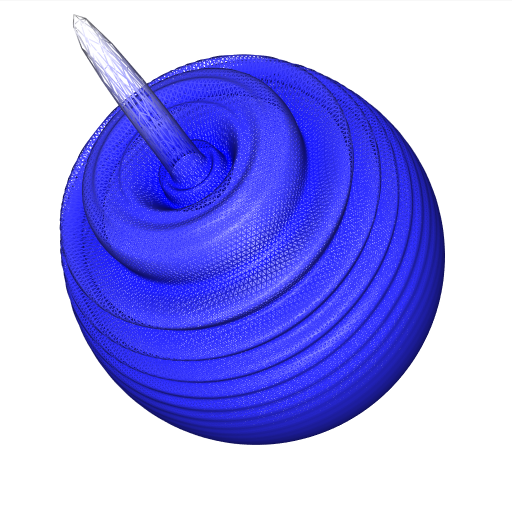
\includegraphics[trim={2.12cm 2.33cm 2.2cm 0cm},clip,width=0.95\textwidth]{images/sphere_wave_7.png}
        \caption{}
      \end{subfigure}
      \caption[Wellensimulation auf einer Kugel]{%
        Die Abbildungen zeigen die Zeitevolution einer Simulation der Wellengleichung auf der gekrümmten Fläche einer Kugel.
        Durch die Geometrie der Kugel existieren keine Ränder und damit auch keine Randbedingungen.
      }
      \label{fig:sphere-wave}
    \end{figure}

  % section conclusion (end)
\end{document}